\documentclass[12pt]{article}
\usepackage{graphicx} % Required for inserting images

\linespread{1.1} % for more than single spacing

% take more advantage of the size of paper
\addtolength{\topmargin}{-2cm}
\addtolength{\textheight}{4cm}
\addtolength{\evensidemargin}{-2cm}
\addtolength{\oddsidemargin}{-2cm}
\addtolength{\textwidth}{4cm}

% some standard packages
\usepackage{booktabs}
\usepackage{mathalpha}
\usepackage{times}
\usepackage{graphics, graphicx}
\usepackage{subfigure, epsfig}
\usepackage{rotate}
\usepackage{tikz, amsmath, amssymb}
\usepackage{enumitem}
\usepackage{hyperref}
\usepackage{float} % for forcing position of figures with H
\usepackage{listings} % for code and output embedding
\lstdefinestyle{mystyle}{
    basicstyle=\ttfamily\footnotesize
}
\lstset{style=mystyle}

% convenient abbreviations
\newcommand{\Cee}{\mathbf{C}}
\newcommand{\Iee}{\mathbf{I}}
\newcommand{\Lee}{\mathbf{L}}
\newcommand{\Ccal}{\mathcal{C}}
\newcommand{\Ical}{\mathcal{I}}
\newcommand{\Lcal}{\mathcal{L}}
\newcommand{\mc}{\multicolumn}
\newcommand{\hs}{\hspace}
\newcommand{\EQ}{\begin{equation}}
\newcommand{\EN}{\end{equation}}
\newcommand{\EQA}{\begin{eqnarray}}
\newcommand{\ENA}{\end{eqnarray}}
\newcommand{\EQAS}{\begin{eqnarray*}}
\newcommand{\ENAS}{\end{eqnarray*}}
\title{CSC311 Report}
\author{Linda Cai, Shizhao Zheng, Yuhan Fu, Yufei Chen}
\date{April 2024}

\begin{document}

\maketitle
\section*{Part A}
\subsection*{1. KNN}
\subsubsection*{(a)}
\begin{figure}[h]
  \centering
  \includegraphics[width=0.5\textwidth]{User_base.jpg}
  \caption{User base}

\end{figure}
 k= 11 is selected and
Validation Accuracy: 0.682613
\subsubsection*{(b)}

The core underlying assumption in item-based collaborative filtering is that if the question A and question B receive same correct and incorrect answers from users who answered them both, then question A is likely to receive same correctness from specific users as question B. This assumption forms the basis for predicting the correctness of answering one question A by some users based on the correctness of answering another question B that is answered similarly with A by other users.

\subsubsection*{(c)}

\begin{figure}[h]
  \centering
  \includegraphics[width=0.5\textwidth]{item_bass.jpg}
  \caption{User base}

\end{figure}

k=21 is selected
Validation Accuracy: 0.692209

\subsubsection*{(d)}

item-based collaborative filtering is better, because Validation Accuracy is 0.692209 doe item-based collaborative filtering, higher than 0.682613 of User-base.\\
I guess this may be the result of our data that questions is much more than users, thus questions have less dimensions and thus we can better distinguish different questions by the inputs. Also we will have more input for questions comparative to the users.
\subsubsection*{(e)}


1.model will be less effective when the scale of data increase\\
As the number of items (questions in this case) and users increases, the dimension of each question will increase dramatically. Then many of the question may be similar to the average case making the model ineffective in distinguishing similarities between item or users. e.g in a case of sparse matrix of 5000*5000, many of the similarities may be close to zero\\
\\
\noindent2.Sparsity may cause our model not reliable\\
In this datasets, user-item interaction matrices is very sparse, meaning that users have interacted with only a small fraction of all items. This sparsity makes it hard to find close neighbors for accurate predictions, especially for less popular items that have limited user interactions. even found one, we are not sure they are really similar enough to meet our assumption.
\newpage
\subsection*{2. Item Response}
\subsubsection*{(a)}
\begin{align*}
p(C|\theta,\beta) &= \prod_{i,j} \left( p(C_{ij}=1|\theta_i,\beta_j) \right)^{C_{ij}} \left(p(C_{ij}=0|\theta_i,\beta_j) \right)^{1 - C_{ij}}
\end{align*}
\begin{align*}
\log p(C|\theta,\beta) &= \sum_{i,j} C_{ij} \log \left( p(C_{ij}=1|\theta_i,\beta_j) \right) + (1 - C_{ij}) \log \left( 1 - p(C_{ij}=1|\theta_i,\beta_j) \right) \\
&= \sum_{i,j} C_{ij} \log \left( \frac{\exp(\theta_i - \beta_j)}{1 + \exp(\theta_i - \beta_j)} \right) + (1 - C_{ij}) \log \left( 1 - \frac{\exp(\theta_i - \beta_j)}{1 + \exp(\theta_i - \beta_j)} \right) \\
&= \sum_{i,j} C_{ij} (\theta_i - \beta_j) - \sum_{i,j} \log(1 + \exp(\theta_i - \beta_j)) \\
&\quad + \sum_{i,j} \log(1 + \exp(\theta_i - \beta_j)) - \sum_{i,j} C_{ij} \log(1 + \exp(\theta_i - \beta_j)) \\
&= \sum_{i,j} C_{ij} (\theta_i - \beta_j) - \sum_{i,j} C_{ij} \log(1 + \exp(\theta_i - \beta_j))\\
&=\sigma(\theta, \beta)
\end{align*}
$$\frac{\partial}{\partial \theta_i} \log p(C|\theta,\beta) = \sum_{j} C_{ij} - \sum_{j} \frac{\exp(\theta_i - \beta_j)}{1 + \exp(\theta_i - \beta_j)}$$
$$\frac{\partial}{\partial \beta_j} \log p(C|\theta,\beta) = - \sum_{i} C_{ij} + \sum_{i} \frac{\exp(\theta_i - \beta_j)}{1 + \exp(\theta_i - \beta_j)}
$$
\subsubsection*{(c)}
I choose iteration number of 40, and learn rate of 0.02 as my final hyper parameters. For the final model, the validation accuracy is 0.70575783234547, and the test accuracy is 0.7067456957380751.\\
\begin{figure}[h]
    \begin{minipage}{0.4\textwidth}
    \centering
    \includegraphics[width=1\textwidth]{vlld.jpg}
    \caption{Validation log likelyhood}
    \label{fig:vlld}
    \end{minipage}%
    \begin{minipage}{0.4\textwidth}
    \centering
    \includegraphics[width=1\textwidth]{tlld.jpg}
    \caption{Test log likelyhood}
    \label{fig:tlld}
    \end{minipage}%
\end{figure}

\newpage
\subsubsection*{(d)}
\begin{figure}[h]
\centering
\includegraphics[width=0.5\textwidth]{pvt.jpg}
\caption{probability vs theta}
\end{figure}
\noindent From the curve, we can see that the method gives good covergence for the three of the probabilities according to theta.The first and second curve converges to above 0.5 shows the two person are likely to answer the question correctly. The third curve converges to below 0.4 shows that the person is likely to answer the question wrong\\
However, the tail of the three curves shows that the initalization of the parameters can be improved so that we can start at closer place to optimal solutions.
\newpage
\subsection*{3. Matrix Factorization}
\subsubsection*{(a)}
I ran SVD with k = 1, 2, 5, 10, 20 and calculated the validation accuracy for each k. The best k was 5 with an accuracy of 0.659046006209427.\\
Validation Accuracy: 0.6428168219023427 with k = 1\\
Validation Accuracy: 0.6579170194750211 with k = 2\\
Validation Accuracy: 0.659046006209427 with k = 5\\
Validation Accuracy: 0.6586226361840248 with k = 10\\
Validation Accuracy: 0.6539655659046006 with k = 20\\
So k = 5 is chosen as the best k,with validation accuracy 0.659046006209427.\\
Best k: 5 with test accuracy: 0.6635619531470506\\

\subsubsection*{(b)}
One limitation of SVD for this task is that it treats missing entries by using mean imputation. However,
mean imputation can introduce noise, especially in sparse regions of the data, as it assumes that missing values are similar
to the mean of the respective item. This might not hold true in reality, especially for different users or items. Therefore,
a limitation of SVD in this case is that it may lead to incorrect estimations of missing values, thereby affecting the quality
of matrix reconstruction.


\subsubsection*{(c \& d)}
After implementing the ALS with SGD, I ran the algorithm with k = 1, 6, 11, 16, 21,lr from 0.01 to 0.25 with step size 0.01, iterations from 1 to 80000 with step size 10000.\\
Finally, I found the best k = 11,lr = 0.06, iterations = 80000 is the best set of hyperparameters.\\
\begin{figure}[h]
\centering
\includegraphics[width=0.5\textwidth]{validation accuracy vs k.jpg}
\caption{validaion accuracy vs k}
\end{figure}

\subsubsection*{(e)}
\begin{figure}[h]
\centering
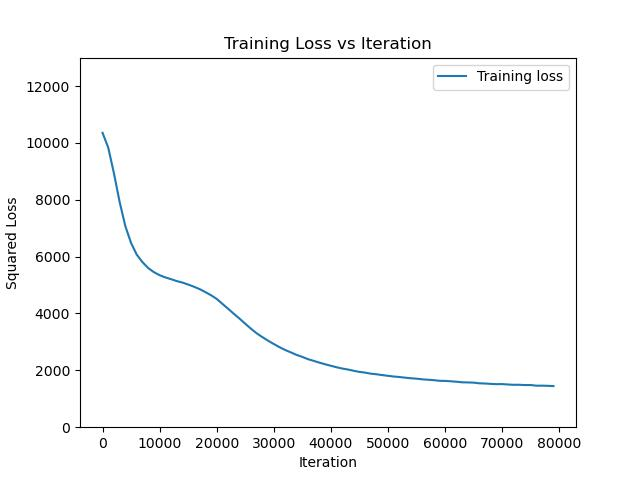
\includegraphics[width=0.5\textwidth]{losses vs iteration.jpg}
\caption{Losses vs Iteration}
\end{figure}
final model is trained with k = 11, lr = 0.06, iterations =80000 with validation accuracy 0.6954558283940163, test accuracy 0.6824724809483489.\\
\newpage
\subsection*{3.Neural networks}
\subsubsection*{a}
1.\textbf{ALS} only decompose the sparse matrix to two matrix and try to reform the original matrix. The model is simple and limited for more complex relationships between inputs and outputs\\
\textbf{Neural Networks}  with nolinear activation functions, can model complex relationships\\
\\
2.\textbf{ALS} decompose the original matrix to two matrix. It only focus on the superficial traits of the matrix\\
\textbf{Neural Network} have a hidden autoencoder layer that will learn the inherent features of inputs which generates more insights into the data.
\\
3.\textbf{ALS} uses iterative alternating optimization for U and Z to obtain the optimizer of U and Z\\
\textbf{Neural Networks} uses backward propagation that goes through two layers of the Neural Networks to obtain optimal $W_1$, $W_2$
\subsubsection*{c}
I choose K of size 50, epoch of number 50 and learn rate of 0.01
\subsubsection*{d}
\begin{figure}[h]
    \begin{minipage}{0.5\textwidth}
    \centering
    \includegraphics[width=1\textwidth]{val_obj.jpg}
    \caption{validation objectives}
    \label{fig:vobj}
    \end{minipage}%
    \begin{minipage}{0.5\textwidth}
    \centering
    \includegraphics[width=1\textwidth]{train_obj.jpg}
    \caption{train objectives}
    \label{fig:tobj}
    \end{minipage}%
\end{figure}
The final test accuracy is 0.679
\subsubsection*{e}
We choose the penalty $\lambda$ = 0.001, with validation accuracy $0.6879762912785775$ and test accuracy $0.677$\\
The model doesn't work better with the L2 regularization.
\newpage
\section*{Part B}
\subsection*{1. Formal Description of Modified Algorithm}
We have chosen two modification to the item response model. The first is using the binary maximum likely hood estimator for each $\theta$ and $\beta$ so that we can have a better initial parameter for each of the question and user.
$$\hat{\theta}_i = \frac{{\text{{number of correct answers by user }} i}}{{\text{{total attempts by user }} i}}$$
$$\hat{\beta}_j = \frac{{\text{{number of correct answers for question }} j}}{{\text{{total attempts for question }} j}}
$$
Also to avoid overfitting of the parameters, I have added a L2 regularization for beta and theta so that we have a loss function calculated by
$$\mathcal{C} = logP(C|\theta,\beta)+\lambda(\theta^2+\beta^2)$$
\subsection*{2. Figures and Diagrams of Modified Algorithm}
Validation log likely hood, Train log likely hood and the graph of probability with respect to theta:
\begin{figure}[h]
    \begin{minipage}{0.4\textwidth}
    \centering
    \includegraphics[width=1\textwidth]{mvlld.jpg}
    \caption{Validation log likelyhood modified}
    \label{fig:vlld}
    \end{minipage}%
    \begin{minipage}{0.4\textwidth}
    \centering
    \includegraphics[width=1\textwidth]{mtlld.jpg}
    \caption{Test log likelyhood modified}
    \label{fig:tlld}
    \end{minipage}%
\end{figure}
\begin{figure}[h]
\centering
\includegraphics[width=0.5\textwidth]{mpvt.jpg}
\caption{probability vs theta modified}
\end{figure}
\newpage
\subsection*{3. Comparing Modified Model with Baseline Model}
\begin{table}[htbp]
    \centering
    \caption{Comparison of Algorithms}
    \begin{tabular}{@{}ccccc@{}}
        \toprule
        \textbf{Iteration} & \textbf{Origie (NLLK)} & \textbf{Origine (Score)} & \textbf{Modified (NLLK)} & \textbf{Modified (Score)} \\ \midrule
        1 & 50708 & 0.5038 & 39678 & 0.5083 \\
        2 & 39693 & 0.6135 & 34420 & 0.6820 \\
        3 & 36619 & 0.6341 & 32806 & 0.6938 \\
        4 & 34882 & 0.6558 & 32116 & 0.7012 \\
        5 & 33639 & 0.6674 & 31546 & 0.7051 \\ \bottomrule
    \end{tabular}
\end{table}
\subsection*{4. Explanation of Model's Performance}
Comparing to the original negative likely hood and score, we can see that with our modified algorithm, the model can achieve convergence to score with 5 iterations. And also, the model gives some closeness gurantees for each theta and beta. comparing to the original probability vs. theta graph, we can see that the initial point is relative closer at most 0.8 where as for original algorithm, it could be 3 unit apart.
\subsection*{5. One Limitation of the Model}
The model assumes a binomial pattern of students answering the question correctly, but in reality, a gaussian model is more appropriate. The core assumption of our model may deviate from more fundamental distribution feature of the input data

\newpage
\section*{Part B}
\subsection*{1. Formal Description of Modified Algorithm}
The first modification is to use the $L^2$ regularization for the ALS with SGD. The loss function is defined as
\begin{align*}
L(U,Z) = \sum_{(n,m) \in O} (C_{nm} - u_n^\top z_m)^2 + \lambda \left( \|U\|_F^2 + \|Z\|_F^2 \right)
\end{align*}
The second modification is decreasing the learning rate dynamically.\\
There is 3 ways to decrease the learning rate dynamically.\\
1. Reduce the learning rate exponentially.\\
\begin{align*}
lr_t = lr_{\text{initial}} * \text{decay\_rate}^{\text{t}}
\end{align*}
2. Reduce the learning rate by Cosine Annealing.\\
\begin{align*}
lr_t = lr_{initial} \times \frac{1 + \cos\left(\frac{\pi \cdot t}{T}\right)}{2}
\end{align*}
3. Reduce the learning rate by Polynomial Decay.\\
\begin{align*}
lr_t = lr_{\text{initial}} \times (1 - \frac{t}{T})^p
\end{align*}
The third attempt is to use the Mini-batch SGD.\\


\subsection*{2. Figures and Diagrams of Modified Algorithm}
\subsubsection*{$L^2$ regularization}
\begin{figure}[h]
\centering
\includegraphics[width=0.5\textwidth]{l2_val_obj.jpg}
\caption{Validation log likelyhood with $L^2$ regularization}
\label{fig:vlld}
\end{figure}
\subsubsection*{Dynamic Learning Rate}
\begin{figure}[h]
    \begin{minipage}{0.4\textwidth}
    \centering
    \includegraphics[width=1\textwidth]{cosine_val_obj.jpg}
    \caption{Validation log likelyhood with Cosine Annealing}
    \label{fig:vlld}
    \end{minipage}%
    \begin{minipage}{0.4\textwidth}
    \centering
    \includegraphics[width=1\textwidth]{cosine_train_obj.jpg}
    \caption{Train log likelyhood with Cosine Annealing}
    \label{fig:tlld}
    \end{minipage}%
\end{figure}
\subsection*{3. Comparing Modified Model with Baseline Model}
\subsection*{4. Explanation of Model's Performance}
\subsection*{5. One Limitation of the Model}

\end{document}
